\documentclass[conference]{IEEEtran}

%+++++++++++++++++++++++++++++++++++++++++++++++++++
\usepackage[pdftex]{graphicx}
\usepackage{amsmath}
\usepackage{eqparbox}
\usepackage[spanish,activeacute]{babel}
\usepackage[utf8x]{inputenc}
\usepackage{graphicx}
%+++++++++++++++++++++++++++++++++++++++++++++++++++

\begin{document}

%+++++++++++++++++++++++++++++++++++++++++++++++++++
\title{\LARGE Creación de un Daemon de Linux usando C y configuración del mismo como un servicio (Servidor Web)}
\author{
\IEEEauthorblockN{\\Instituto Tecnológico de Costa Rica}
\IEEEauthorblockN{\\Área Académica de Ingeniería en Computadores}
\IEEEauthorblockN{\\ CE-4303 Principios de sistemas operativos}
\IEEEauthorblockN{\\Bryan Abarca Weber}
\IEEEauthorblockN{Raúl Arias Quesada}
\IEEEauthorblockN{Rony Paniagua Chacón}
}
%+++++++++++++++++++++++++++++++++++++++++++++++++++

\maketitle

% ========================
% # I. Introducción      #
% ========================

\section{Introducción}
El presente documento tiene como finalidad presentar la solución a la tarea corta 1, la cual consiste en la creación de un web server en el lenguaje C y convertirlo en un servicio daemon en el sistema operativo Linux.
\\\\Un daemon o demonio es un proceso que se ejecuta en segundo plano, no se conecta a ninguna terminal de control. Estos normalmente se inician en el momento del arranque mediante scripts de SysV init que se encuentran comúnmente en /etc/init.d o /etc/rc.d o con scripts de systemd (dependiendo del sistema). Cuando la máquina bootea se corre el primer proceso (init o systemd) el cual se encarga de levantar todos los daemons (que a su vez estos pueden levantar otros daemons) que deben ejecutarse al comienzo del funcionamiento del sistema. Pero no todos son configurados para iniciar en la secuencia de booteo, si no que también pueden ser iniciados manualmente por el usuario desde la consola de comandos del sistema, o por otros daemons que bajo cierta configuración se ejecutan en determinado momento. Los daemons se ejecutan como root o algún otro usuario especial (como apache o postfix), y se encargan de las tareas a nivel del sistema [1].
\\Estos tienen dos requerimientos generales: tienen que correr como un hijo de init (primer proceso que se ejecuta en Linux) y no deben estar conectados a la terminal [1].
\\En [1] se describen los siguientes pasos para que un programa se convierta en un Daemon:
\begin{enumerate}
    \item Llama a fork (). Esto crea un nuevo proceso, que se convertirá en el demonio.
    \item Cambia le file mode mask (umask) por si necesita escribir en cualquier archivo (incluidos los registros) creados por el demonio y así asegurarse de que puedan escribirse o leerse correctamente.
    \item En el padre, llama a exit (). Esto garantiza que el padre original (el abuelo del daemon) esté satisfecho de que su hijo haya terminado, que el padre del daemon ya no se esté ejecutando y que el daemon no sea un líder de grupo de procesos. Este último punto es un requisito para la finalización exitosa del siguiente paso.
    \item Llama a setsid (), dando al demonio un nuevo proceso de grupo y sesión, los cuales lo tienen como líder. Esto también garantiza que el proceso no tenga un terminal de control asociado (ya que el proceso acaba de crear una nueva sesión y no asignará uno).
    \item Cambia el directorio de trabajo al directorio raíz a través de chdir (). Esto se hace porque el directorio de trabajo heredado puede estar en cualquier parte del sistema de archivos. Los demonios tienden a ejecutarse durante el tiempo de actividad del sistema, y no desea mantener abierto un directorio aleatorio y, por lo tanto, evitar que un administrador desmonte el sistema de archivos que contiene ese directorio.
    \item Cierra todos los descriptores de archivos. Ya que no se desea heredar descriptores de archivos abiertos y, sin saberlo, mantenerlos abiertos.
    \item Abre los descriptores de archivo 0, 1 y 2 (standard in, standard out y standard error) y los redirige a /dev/null.
\end{enumerate}
En muchos sistemas de Linux estos pasos son automatizados con funciones propias del sistema. Por ejemplo la función daemon(), que realiza este proceso.
\\\\Los daemons son utilizados con gran variedad de objetivos, por mencionar los más conocidos [3]:
\begin{enumerate}
    \item Existen daemons como servicios que están escuchando solicitudes en puertos, como el www daemon; o para funcionalidades relacionadas con aplicaciones de internet, como el manejo de correos (sendmail daemon, finger daemon, talk daemon, etc.).
    \item También son útiles para la administración del sistema, como estar verificando que no haya errores en el sistema, monitoreando el estado de los componentes (por ejemplo, temperatura), gestión de registros de archivos, limpieza diaria del sistema de archivos, administración de bases de datos, entre otros.
    \item Otro empleo es para responder a solicitudes de archivos por parte de los clientes o componentes del sistema (por ejemplo, los que se encargan de la asignación de puertos), o para programas que son necesarios que estén ejecutándose en todo momento, incluso cuando no se haya iniciado sesión con algún usuario.
    \item Algunas partes del Kernel gestionan como si fueran procesos de usuarios, para lo que se emplean daemons. En su mayor parte estos procesos se encargan de aspectos con dispositivos de E/S, gestión de memoria y sincronización del caché de disco. Estos no pueden ser manipulados por el administrador del sistema, si no que se dejan por su propia cuenta.
    \item Algunos daemons de vital importancia cumplen con funciones de alta responsabilidad, como la administrar otros daemons o servicios del sistema.
    \item Los usuarios también pueden crear daemons para mantener programas corriendo con un objetivo específico sin necesidad de estar iniciándolos manualmente.
\end{enumerate}

Con los administradores de servicios systemctl o service (los cuales también son daemons), dependiendo de cómo la distribución de Linux hace uso de systemd o init, es posible acceder a 4 principales funciones para los daemons [4]:
\begin{itemize}
    \item start: comienza a ejecutarse el Daemon.
    \item stop: cuando el daemon se está ejecutando, es detenido.
    \item restart: cuando el daemon se está ejecutando, es detenido y luego es iniciado nuevamente.
    \item status: indica el estado del daemon, si este está ejecutándose.
\end{itemize}
En cuanto a su funcionamiento, es un programa que está corriendo constantemente en background, y se inicia automáticamente en el arranque de la máquina, para realizar alguna acción, por ejemplo, estar pendiente de solicitudes de recursos o algún servicio, como los recursos web. 
\\Sin embargo, hay daemons que se ejecutan solo por algún tiempo, por ejemplo, el cron daemon, el cual se ejecuta una vez cada minuto, valida si hay alguna acción que deba realizar, si es así ejecuta el trabajo, si no vuelve a “dormir” hasta que sea tiempo para la siguiente validación [2].
\\Hay algunas convenciones comunes que son seguidas por daemons en el sistema UNIX [5].
\begin{itemize}
    \item Las opciones de configuración generalmente se almacenan en /etc: El archivo de configuración se llama name.conf, donde nombre es el nombre del daemon o el servicio. Por ejemplo, la configuración para el syslogd daemon suele ser /etc/syslog.conf.
    \item Si un daemon tiene un archivo de configuración, el daemon lee el archivo cuando se inicia y no lo vuelve a ver. Si un administrador cambia la configuración, el daemon deberá detenerse y reiniciarse para tener en cuenta los cambios de configuración. 
\end{itemize}
El servidor web debe ejecutarse como un servicio de Linux, esto se puede lograr utilizando SysVinit o Systemd. A continuación se presentan sus principales características.
\\\textbf{Systemd}
\\El conjunto de herramientas de systemd proporciona un modelo de inicio rápido y flexible para administrar una máquina completa desde el boot en adelante.
\\Algunas características de Systemd se listan a continuación:
\begin{enumerate}
    \item Systemd proporciona capacidades de paralelización agresivas.
    \item Utiliza la activación de socket y D-Bus para iniciar los servicios.
    \item Ofertas a pedido de arranque de demonios.
    \item Realiza un seguimiento de los procesos utilizando Linux cgroups.
    \item Soporta snapshotting y restauración del estado del sistema
    \item Mantiene los puntos de montaje y automontaje.
    \item Implementa una lógica de control de servicio basada en dependencia transaccional elaborada
\end{enumerate}
El objeto básico que systemd maneja y sobre el que actúa es una unidad. Las unidades pueden ser de muchos tipos, pero el tipo más común es un servicio (indicado por un archivo de unidad que termina en .service). Para administrar los servicios, en un servidor habilitado para systemd, la herramienta principal es el comando systemctl [6].
\\Systemd tiene un concepto de objetivos (targets) que tienen un propósito similar a los niveles de ejecución pero que actúan de manera un poco diferente [8]. De [7] se obtiene la información del siguiente cuadro:

\begin{table}[ht]
\centering
\caption{Systemd targets}
\begin{tabular}{|c|c|}
\hline
\textbf{Objetivo (target)} & \textbf{Descripción} \\ \hline
poweroff & Apagar (entrar en el nivel de ejecución 0) \\ \hline
rescue & Entrar en modo de rescate (nivel de ejecución 1, usuario único)\\ \hline
multi-user & Entrar en modo multiusuario (niveles de ejecución 2 a 4) \\ \hline
graphical & Entrar en modo gráfico (nivel de ejecución 5) \\ \hline
reboot & Reiniciar el sistema (nivel de ejecución 6)\\ \hline
\end{tabular}
\end{table}

Todos los comandos normales del sistema init tienen acciones equivalentes con el comando systemctl. Para demostrar los comando utilizados por systemd se toma como ejemplo el nombre del servicio que se crea en la presente tarea, WebServer [6]. De [6] se obtienen los siguientes comandos.
\begin{itemize}
\item Para iniciar manualmente el servicio se utiliza el comando:
\\systemctl start WebServer
\item Para detener el servicio se utiliza el comando:
\\systemctl stop WebServer
\item Para reiniciar el servicio se ejecuta:
\\systemctl restart WebServer
\item Para intentar recargar el servicio sin interrumpir la funcionalidad normal, se ejecuta:
\\systemctl reload WebServer
\end{itemize}
Por defecto, la mayoría de los archivos de unidades del sistema no se inician automáticamente en el arranque. Para configurar esta funcionalidad, debe habilitar a la unidad. Esto lo conecta a un cierto objetivo de arranque, lo que hace que se active cuando se inicie ese objetivo [6].
\begin{itemize}
\item Para permitir que un servicio se inicie automáticamente en el arranque, se ejecuta:
\\systemctl enable WebServer
\item Si desea volver a desactivar el servicio:
\\systemctl disable WebServer
\end{itemize}
Con systemd se puede tener acceso al estado general del sistema y también se puede obtener información sobre el estado de las unidades individuales.
\begin{itemize}
\item Para obtener una visión general del estado del sistema se ejecuta (unidades que systemd ha listado como activos):
\\systemctl list-units
\item Para ver un resumen del estado actual de una unidad:
\\systemctl status WebServer

\end{itemize}
\textbf{SysVinit o Sys-V}
\\System V (Sys-V) es uno de los primeros y tradicionales sistemas de inicio para Unix como sistema operativo [8].
\\La idea central de Sys-V se basa en los llamados niveles de ejecución, que son esencialmente una forma de organizar una colección de scripts de inicio que deben ejecutarse cuando el sistema se inicia o se apaga. Cada nivel de ejecución corresponde a un directorio en / etc /, que a su vez contiene enlaces simbólicos a scripts en /etc/init.d/ [9].
\\La siguiente tabla obtenida de [9], presenta los principales niveles de ejecución de Sys-V.

\begin{table}[ht]
\centering
\caption{Niveles de ejecución de Sys-V}
\begin{tabular}{|c|c|c|}
\hline
\textbf{Nivel} & \textbf{Directorio} & \textbf{Uso} \\ \hline
N &   & Arranque del sistema \\ \hline
0 & /etc/rc0.d/ & Detener el sistema \\ \hline
1 & /etc/rc1.d/ & Modo de usuario único \\ \hline
2 & /etc/rc2.d/ & Modo multiusuario \\ \hline
3-5 & /etc/rc3.d/ al /etc/rc5.d/ & Idéntico al nivel de ejecución 2 \\ \hline
6 & /etc/rc6.d/ & Reinicio del sistema \\ \hline
\end{tabular}
\end{table}
De igual manera como se demostró el uso de los comando de Systemd, se utilizará el servicio WebServer para demostrar el uso de los comandos de Sys-V. Hay muchas herramientas de línea de comandos que puede utilizar para administrar los servicios de Sys V como los siguientes.
\begin{itemize}
\item Para iniciar manualmente el servicio se utiliza el comando:
\\service WebServer start
\item Para detener el servicio se utiliza el comando:
\\service WebServer stop
\item Para reiniciar el servicio se ejecuta:
\\service WebServer restart
\item El siguiente comando lista los servicios que están activos
\\service --status-all
\item Para ver el estado actual del servicio
\\service WebServer status
\item Para permitir que un servicio se inicie automáticamente en el arranque, se ejecuta:
\\chkconfig WebServer on
\item Si desea volver a desactivar el servicio.
\\chkconfig WebServer off
\end{itemize}
Systemd se está convirtiendo lentamente en el estándar emergente para init, esta es una de las razones por la cual el grupo opta por este sistema para la manipulación del servicio WebServer implementado. 
\\A continuación se presentan otras ventajas, según [7], del uso de Systemd.

\begin{itemize}
\item Los daemons de Systemd facilitan la supervisión y el control de los procesos y la ejecución de trabajos paralelos.
\item Systemd ofrece el comando systemctl y cgroups para hacer su vida más fácil:
\begin{itemize}
\item systemctl proporciona al administrador mensajes de error más detallados, incluidos los errores de tiempo de ejecución y de inicio.
\item cgroups, o "grupos de control", permiten agrupar los procesos en una jerarquía para facilitar la administración.
\end{itemize}
\item Los atributos del proceso, como la función y la propiedad, son mucho más fáciles de determinar. Por ejemplo, bajo Systemd, los subprocesos, una vez generados, se convierten en children y se organizan bajo el grupo parent apropiado para mostrar la herencia.
\end{itemize}
\textbf{Runlevels vs targets}
\\Systemd tiene el concepto de target para reemplazar el concepto clásico de runlevel de los sistemas Sys-V. Un target es similar a un runlevel, con algunas diferencias. Algunos targets incluso se crean y heredan los servicios de otro target, y a su vez, puede agregar servicios nuevos [10].
\\Un target tiene un nombre, no un número como los runlevels, y está orientado a un uso específico. Al ser un concepto equivalente al de runlevel, se puede utilizar init o telinit para intercambiar los targets en el sistema, tal cual se hacía en Sys-V con los números de runlevel [10].
\\Los targets son directorios que se encuentran generalmente en /etc/systemd/system/ y tienen nombres similares a “mitarget.target.wants”. Dentro del directorio de un target se linkean como symlink (ln -s) los archivos de servicio que se encuentran por lo general en /lib/systemd/system/y son archivos de servicios con “extensión” .service [10].

% =============================================
% # II. Ambiente de desarrollo utilizado      #
% =============================================

\section{Ambiente de desarrollo utilizado}
Para el desarrollo de este proyecto fueron necesarias las herramientas:
\begin{enumerate}
    \item Sistema operativo con distribución LInux preferiblemente Ubuntu.
    \item Editor de código C, incluso puede ser utilizado el editor de texto del sistema operativo, en nuestro caso utilizamos el editor libre Visual Studio Code. 
\end{enumerate}

% =============================================
% # III. Estructuras, funciones y librerías   #
% =============================================
\newpage
\section{Estructuras, funciones y librerías}
\begin{figure}[ht!] 
\centering
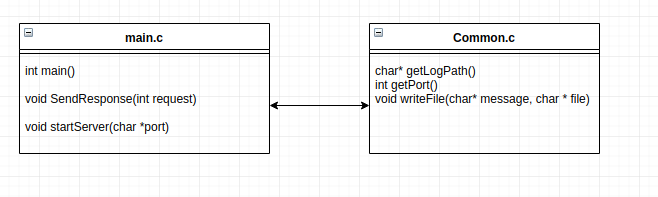
\includegraphics[width=3.4in]{diagrama.png}
\caption{Diagrama de la solución.}
\end{figure}
El proyecto cuenta con dos archivos el main.c donde se instancia y crea el web server y el archivo Common,c con funciones comunes para la lectura y escritura de datos en un archivo, basado en [11].
\\En el archivo main se encuentran los métodos:
\begin{enumerate}
    \item startServer: este método recibe como entrada el puerto, se encarga de levantar el servidor web, ejecutando las acciones socket y bind del servidor, esto utilizando la librería sys/socket.h.
    \item SendResponse: Recibe como entrada el request a contestar, se encarga de verificar el request y responder utilizando HTTP-1.1 para ello ejecuta métodos como recv para leer el request y write para responder.
    \item main: Método principal encargado de leer los valores de los archivos de configuración, levantar el servidor y se mantiene escuchando y aceptando conexiones est utilizando los otros métodos creados.
\end{enumerate}
En el archivo Common se encuentran los métodos: 
\begin{enumerate}
    \item getLogPath: Método que lee el archivo de configuración y devuelve el path para el archivo donde escribir los logs, para ello busca la linea que tenga el valor de “LOGFILE”, en caso de no encontrar el valor del path devuelve el valor por defecto /var/log/syslog. Utiliza métodos como fopen para abrir el archivo, fgets para leer líneas del archivo y sscanf para buscar la línea correcta.
    \item getPort: Método que lee el archivo de configuración y devuelve el puerto a utilizar, para ello busca la linea que tenga el valor de “PORT”, en caso de no encontrar el valor del puerto devuelve el valor por defecto 8081. Utiliza métodos como fopen para abrir el archivo, fgets para leer líneas del archivo y sscanf para buscar la línea correcta. 
    \item write: Recibe los datos a escribir y la ruta del archivo donde escribir, además de escribir el mensaje requerido escribe la hora del sistema para tener un mejor log de la actividad. Utiliza la librería time.h para obtener la hora y métodos como fopen para abrir el archivo y fprintf para escribir en él. 
\end{enumerate}

% ==============================
% # IV. Instrucciones de uso   #
% ==============================

\section{Instrucciones de uso}
Pasos previos a compilar el proyecto: 
\begin{enumerate}
    \item Cambiar la ruta donde se ubicará el archivo ejecutable, esto modificando el archivo WebServer.service, dentro del archivo modificar el parámetro ExecStart, por la ruta donde se encuentra la carpeta WebServerDir.
    \item Dar permisos de escritura al archivo /var/log/syslog en caso de utilizar el archivo por defecto.
    \item Ajustar el archivo config.conf con el valor del puerto y archivo donde registrar el log.
\end{enumerate}
Compilar la tarea con el comando make desde una terminal ubicada en la ruta donde está el archivo Makefile entregado. Con esto el servicio estará funcionando.
\\Para utilizar el servicio se deben pegar los archivos a mostrar en la carpeta WebServerDir y podrán ser accesados desde un navegador web en la ruta localhost:puerto/nombreArchivo/extensión
//Para interactuar con el servicio se pueden usar los comandos de una terminal:
\begin{itemize}
    \item sudo systemctl start WebServer: Para iniciar el servicio.
    \item sudo systemctl stop WebServer: Para detener el servicio.
    \item sudo systemctl restart WebServer: Reinicia el servicio.
    \item sudo systemctl status WebServer: Para obtener el estado del servicio
\end{itemize}
Adicionalmente se brinda el archivo UnistallWebServer.sh para remover el servicio, el cual se puede utilizar ejecutando el comando: sh UnistallWebServer.sh esto desde una terminal en la ubicación del archivo.

% ================
% # V. Bitácora  #
%=================

\section{Bitácora}
A continuación se presenta el registro de las actividades de cada estudiante:

\begin{table}[ht]
\centering
\caption{Bitácora Bryan Abarca}
\begin{tabular}{|c|c|}
\hline
\textbf{Actividad} & \textbf{Tiempo} \\ \hline
Análisis de la tarea. & 30 min \\ \hline
Investigación servicios en linux. & 2 h\\ \hline
Desarrollo y pruebas del servicio. & 1 h\\ \hline
Ajustes al entregable, makefile, estructura de carpetas. & 1 h\\ \hline
Documentación. & 3 h\\ \hline
Total & 7 h 30 min\\ \hline

\end{tabular}
\end{table}

\begin{table}[ht]
\centering
\caption{Bitácora Raúl Arias}
\begin{tabular}{|c|c|}
\hline
\textbf{Actividad} & \textbf{Tiempo} \\ \hline
Análisis de la tarea. & 30 min \\ \hline 
Investigación web server. & 2 h  \\ \hline
Investigación servicios en linux & 1 h \\ \hline
Desarrollo web server básico. & 2 h \\ \hline
Documentación. & 2 h \\ \hline
Total & 7 h 30 min \\ \hline
\end{tabular}
\end{table}

\begin{table}[ht]
\centering
\caption{Bitácora Rony Paniagua}
\begin{tabular}{|c|c|}
\hline
\textbf{Actividad} & \textbf{Tiempo} \\ \hline
Análisis de la tarea. & 30 min \\ \hline
Investigación ajustes web server(leer config, escribir logs). & 2 h\\ \hline
Investigación servicios en linux. & 1 h\\ \hline
Desarrollo ajustes web server. & 1 h\\ \hline
Ajustes al entregable, makefile, estructura de carpetas. & 1 h\\ \hline
Documentación. & 3 h\\ \hline
Total & 8 h 30 min\\ \hline
\end{tabular}
\end{table}

% ====================
% # V. Conclusiones  #
%=====================

\section{Conclusiones}

Al finalizar el trabajo se puede concluir que la implementación de daemons automatiza la ejecución de programas o servicios que son necesarios para el sistema, así el usuario no debe hacerse responsable de esta tarea, y se evita que estos programas estén ligados a una terminal, con lo que se previene que no sean detenidos por un tercero.
\\Además, Linux brinda la posibilidad a los programadores a instalar sus propios daemons y configurarlos a gusto, ya sea que se ejecuten en la secuencia de booteo junto con los demás daemons del sistema o que se inicien manualmente. Así se pueden crear programas o servicios que se ejecuten por defecto, como el caso de esta investigación, un servidor web personalizado.
\\Según lo investigado, el sistema de inicio SysV no posee ciertas características que son necesarias para la computación moderna, y debido a decisiones de diseño fundamentales, estas características son esencialmente imposibles de volver a ajustar en ellas. Por otro lado, Systemd es una característica completa para todos estos requerimientos y se adapta bien al hardware moderno.


% =======================
% # V. Recomendaciones  #
%========================

\section{Recomendaciones}
Utilizar un editor de código C que facilite la escritura de código, detectando errores y proporcionando autocompletado.
\\Emplear el uso de alguna herramienta de generación o automatización de código como por ejemplo GNU Make. El objetivo general de las herramientas de construcción es automatizar el proceso de generación y/o actualización de un conjunto de ficheros (objetivo) que se construyen a partir de otros (fuente). Y no sólo automatizarlo, sino hacerlo de manera eficiente.

% ====================
% # V. Referencias  #
%=====================

\begin{thebibliography}{1}
\bibitem{}
R. Love. Linux System Programming. 1ra. Ed. California, USA: O'Reilly Media, Inc, septiembre, 2007.
\bibitem{}
P. Anderson.(septiembre, 1994). Towards a High-Level Machine
Configuration System. [En línea]. Disponible en: http://www.lcfg.org/doc/LISA8\_Paper.pdf
\bibitem{}
E. Nemeth, G. Snyder, T. R. Hein. 2da Ed. Massachusetts, USA: Pearson Education, Inc, octubre, 2007.
\bibitem{}
M. Van Canneyt. (febrero, 2007). Taming the daemon: Writing cross-platform service applications in FPC/Lazarus. [En línea]. Disponible en: https://www.freepascal.org/~michael/articles/daemons/daemons.pdf
\bibitem{}
Chapter 13. Daemon Processes. Shichao’s Notes. [En línea]. Disponible en: https://notes.shichao.io/apue/ch13/
\bibitem{}
J. Ellingwood (Abril, 2015) Systemd Essentials: Working with Services, Units, and the Journal. [En línea]. Disponible en: https://www.digitalocean.com/community/tutorials/systemd-essentials-working-with-services-units-and-the-journal 
\bibitem{}
A. Anderson (Mayo, 2017). Advantages of Systemd vs. SysVinit, with Example Commands. [En línea]. Disponible en: https://kernelmastery.com/systemd-vs-sysvinit/
\bibitem{}
P. Subramanian. (Febrero, 2016). SysVinit Vs Systemd Cheatsheet. [En línea]. Disponible en: https://www.2daygeek.com/sysvinit-vs-systemd-cheatsheet-systemctl-command-usage/
\bibitem{}
B. Bearnes. (Septiembre, 2015). SysV init: Runlevels. [En línea]. Disponible en: https://learn.adafruit.com/running-programs-automatically-on-your-tiny-computer/sysv-init-runlevels
\bibitem{}
D. Córdoba. (Marzo, 2016). Systemd vs Sysvinit: Algunos comandos. [En línea]. Disponible en: https://juncotic.com/comandos-sysvinit-vs-comandos-systemd/
\bibitem{}
Rastogi, A. (2010). A Very Simple HTTP Server writen in C. [En línea] Abhijeet's Blog. DIsponible en: https://blog.abhijeetr.com/2010/04/very-simple-http-server-writen-in-c.html.
\end{thebibliography}


\end{document}